\documentclass{article}
\usepackage[margin=1in]{geometry}
\usepackage{graphicx}
\usepackage{xcolor}
\usepackage{float}
\usepackage{amsmath}
\usepackage{cite}
\usepackage{hyperref}
\graphicspath{{..} {./images}}

\definecolor{navy-blue}{rgb}{0.22,0.38,0.71}

\renewcommand{\contentsname}{\vspace*{-2\baselineskip}}

\hypersetup{
	colorlinks,
	linkcolor=black,
	urlcolor=black,
	citecolor=black
}
  		
\begin{document}
\begin{titlepage}
	\centering
	{\huge Lab 2 - Introduction to Software-Defined Radio}\\[0.25 in]
	
\includegraphics[width=0.6\textwidth]{ua_logo.png}\\[0.25 in]
	{\large \textbf{ECE 531 - Software Defined Radio\\[0.25 in]
	February 26, 2025\\[0.25 in]}}
	{\large Owen Sowatzke, osowatzke@arizona.edu\\[0.05 in]
	Department of Electrical \& Computer Engineering\\[0.05 in]
	University of Arizona, Tucson, AZ 85721\\[0.5 in]}
	\hypersetup{linkcolor=navy-blue}
	\noindent\hrulefill
	\tableofcontents
	\noindent\hrulefill
\end{titlepage}

\setlength{\parindent}{0pt}

\section{Introduction}
%Introduction to the laboratory experiment, including a brief description of the objectives and goals.

\section{Procedure}
% Detailed explanation of the laboratory experiment, including the design, implementation, and testing of the system.

\subsection{Industrial Input/Output (IIO)}
\label{section::industrial_input_output}

We can use the \texttt{iio\_info -s} command to identify the PlutoSDR device's Universal Resource Identifier (URI). We execute the provided command in an SSH terminal session connected to the embedded PlutoSDR operating system and in a local PC terminal. After executing the command in both terminals, we compare the resulting URIs.

Next, we use the \texttt{iio\_attr} command in the SSH terminal to locate the \textit{ad9361-phy} device. Once we find the device, we use the following command to verify the device name:

\begin{center}
\texttt{cat /sys/bus/iio/devices/$<$iio\_device$>$/name}
\end{center}

where \texttt{$<$iio\_device$>$} is the IIO device we find with the \texttt{iio\_attr} command. Then, we use the \texttt{iio\_attr} command to list the attributes of the \textit{ad9361-phy} device.


\section{Results}
\subsection{Industrial Input/Output (IIO)}

In this section, we display the results from the industrial input/output commands provided in Section \ref{section::industrial_input_output}. Figure \ref{fig::iio_info_putty} displays the results of the \texttt{iio\_info -s} command, when executed in Putty (an SSH terminal).  

\begin{figure}[H]
	\centerline{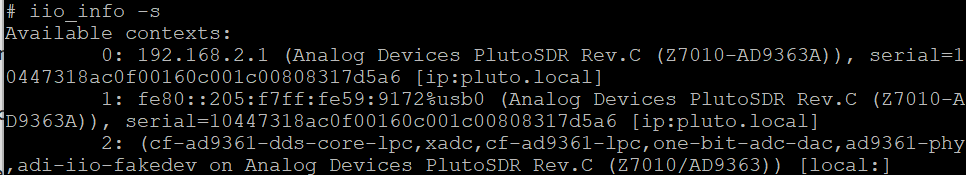
\includegraphics[width=0.9\textwidth]{iio_info_putty.png}}
	\caption{Result of \texttt{iio\_info -s} Command when Executed in Putty}
	\label{fig::iio_info_putty}
\end{figure}

Figure \ref{fig::iio_info_cmd} shows the outputs of the same command when executed in command prompt, a local PC terminal.

\begin{figure}[H]
	\centerline{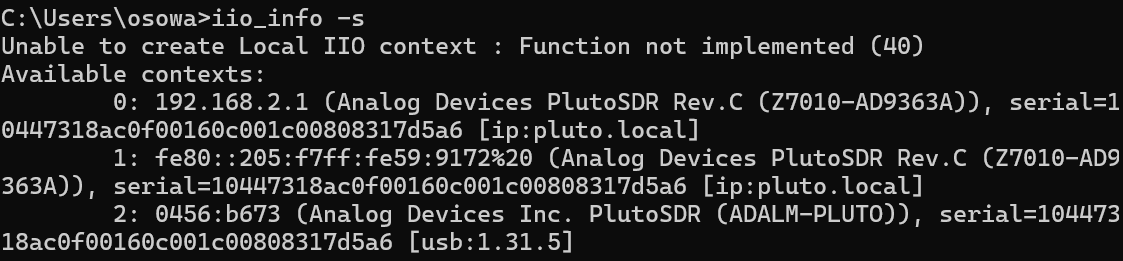
\includegraphics[width=0.9\textwidth]{iio_info_cmd.png}}
	\caption{Result of \texttt{iio\_info -s} Command when Executed in Command Prompt}
	\label{fig::iio_info_cmd}
\end{figure}

Compared to the outputs shown in Figure \ref{fig::iio_info_putty}, the command prompt output shows very similar URIs. Both contain an ip:pluto.local URI with an IP address of 192.168.2.1. They also both contain an additional ip:pluto.local URI, which is nearly the same. However, the biggest difference between the two outputs is in the final URI. The SSH output shows a local URI (local:), while the command prompt output shows a USB URI (usb:1.31.5). We note that command prompt also contains an additional warning message, which says "Unable to create Local IIO context: Function not implemented (40)." This warning message is described in more detail in \cite{analog_devices_libiio_error}. However, it is expected warning because \texttt{iio\_info} tries to open local contexts, which are not supported in Windows. For comparison, we run the same command on the Virtual Machine. The results of this command are display in Figure \ref{fig::iio_info_vm}.

\begin{figure}[H]
	\centerline{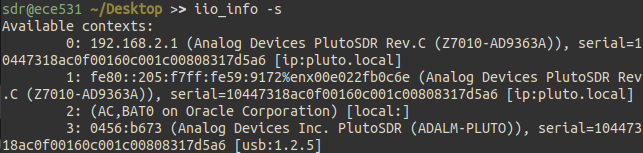
\includegraphics[width=0.9\textwidth]{iio_info_vm.png}}
	\caption{Result of ``iio\_info -s" Command when Executed in Virtual Machine}
	\label{fig::iio_info_vm}
\end{figure}

\begin{figure}[H]
	\centerline{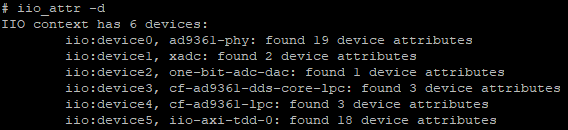
\includegraphics[width=0.75\textwidth]{iio_devices.png}}
	\caption{List of IIO Devices}
	\label{fig::iio_devices}
\end{figure}

\begin{figure}[H]
	\centerline{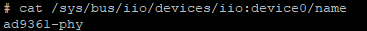
\includegraphics[width=0.5\textwidth]{iio_device0_name.png}}
	\caption{Confirming Name of ``iio:device0"}
	\label{fig::iio_device0_name}
\end{figure}

\begin{figure}[H]
	\centerline{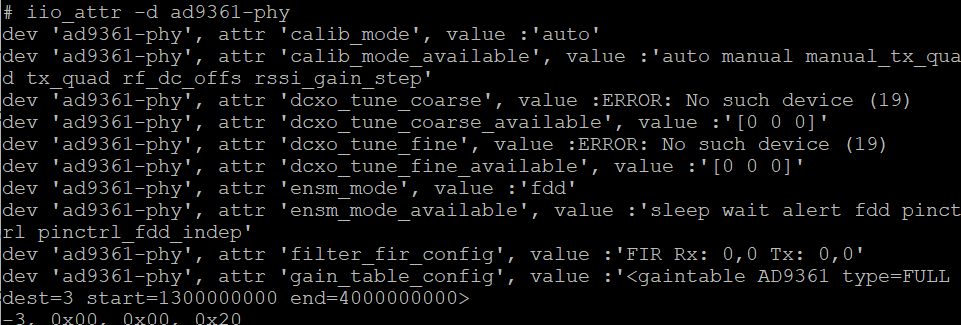
\includegraphics[width=0.9\textwidth]{iio_raw_attributes.png}}
	\caption{Attributes for ``ad9361-phy" Device}
	\label{fig::iio_raw_attributes}
\end{figure}

\begin{figure}[H]
	\centerline{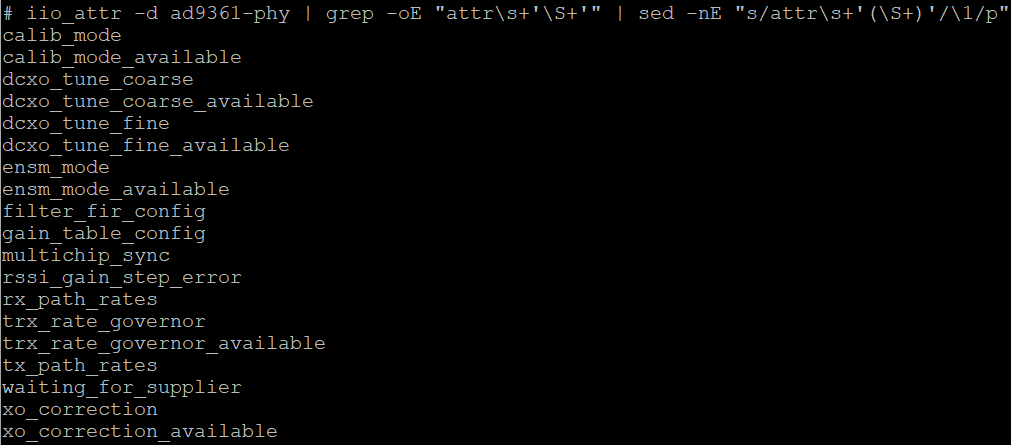
\includegraphics[width=0.9\textwidth]{iio_filtered_attributes.png}}
	\caption{Filtering Output of "iio\_attr" Command}
	\label{fig::iio_filtered_attributes}
\end{figure}
% Results and discussion of the laboratory experiment, including captured outputs, observations, and responses to laboratory questions.

\section{Conclusion}
% Conclusions to the overall lab that discuss meaningful lessons learned and other takeaways from the assignment. (Important)

\nocite{analog_devices_libiio_error}
\bibliographystyle{IEEEtran}
\bibliography{sources}{}
%\bibliographystyle{ieeetr}
	
\end{document}